\documentclass[1p]{elsarticle_modified}
%\bibliographystyle{elsarticle-num}

%\usepackage[colorlinks]{hyperref}
%\usepackage{abbrmath_seonhwa} %\Abb, \Ascr, \Acal ,\Abf, \Afrak
\usepackage{amsfonts}
\usepackage{amssymb}
\usepackage{amsmath}
\usepackage{amsthm}
\usepackage{scalefnt}
\usepackage{amsbsy}
\usepackage{kotex}
\usepackage{caption}
\usepackage{subfig}
\usepackage{color}
\usepackage{graphicx}
\usepackage{xcolor} %% white, black, red, green, blue, cyan, magenta, yellow
\usepackage{float}
\usepackage{setspace}
\usepackage{hyperref}

\usepackage{tikz}
\usetikzlibrary{arrows}

\usepackage{multirow}
\usepackage{array} % fixed length table
\usepackage{hhline}

%%%%%%%%%%%%%%%%%%%%%
\makeatletter
\renewcommand*\env@matrix[1][\arraystretch]{%
	\edef\arraystretch{#1}%
	\hskip -\arraycolsep
	\let\@ifnextchar\new@ifnextchar
	\array{*\c@MaxMatrixCols c}}
\makeatother %https://tex.stackexchange.com/questions/14071/how-can-i-increase-the-line-spacing-in-a-matrix
%%%%%%%%%%%%%%%

\usepackage[normalem]{ulem}

\newcommand{\msout}[1]{\ifmmode\text{\sout{\ensuremath{#1}}}\else\sout{#1}\fi}
%SOURCE: \msout is \stkout macro in https://tex.stackexchange.com/questions/20609/strikeout-in-math-mode

\newcommand{\cancel}[1]{
	\ifmmode
	{\color{red}\msout{#1}}
	\else
	{\color{red}\sout{#1}}
	\fi
}

\newcommand{\add}[1]{
	{\color{blue}\uwave{#1}}
}

\newcommand{\replace}[2]{
	\ifmmode
	{\color{red}\msout{#1}}{\color{blue}\uwave{#2}}
	\else
	{\color{red}\sout{#1}}{\color{blue}\uwave{#2}}
	\fi
}

\newcommand{\Sol}{\mathcal{S}} %segment
\newcommand{\D}{D} %diagram
\newcommand{\A}{\mathcal{A}} %arc


%%%%%%%%%%%%%%%%%%%%%%%%%%%%%5 test

\def\sl{\operatorname{\textup{SL}}(2,\Cbb)}
\def\psl{\operatorname{\textup{PSL}}(2,\Cbb)}
\def\quan{\mkern 1mu \triangleright \mkern 1mu}

\theoremstyle{definition}
\newtheorem{thm}{Theorem}[section]
\newtheorem{prop}[thm]{Proposition}
\newtheorem{lem}[thm]{Lemma}
\newtheorem{ques}[thm]{Question}
\newtheorem{cor}[thm]{Corollary}
\newtheorem{defn}[thm]{Definition}
\newtheorem{exam}[thm]{Example}
\newtheorem{rmk}[thm]{Remark}
\newtheorem{alg}[thm]{Algorithm}

\newcommand{\I}{\sqrt{-1}}
\begin{document}

%\begin{frontmatter}
%
%\title{Boundary parabolic representations of knots up to 8 crossings}
%
%%% Group authors per affiliation:
%\author{Yunhi Cho} 
%\address{Department of Mathematics, University of Seoul, Seoul, Korea}
%\ead{yhcho@uos.ac.kr}
%
%
%\author{Seonhwa Kim} %\fnref{s_kim}}
%\address{Center for Geometry and Physics, Institute for Basic Science, Pohang, 37673, Korea}
%\ead{ryeona17@ibs.re.kr}
%
%\author{Hyuk Kim}
%\address{Department of Mathematical Sciences, Seoul National University, Seoul 08826, Korea}
%\ead{hyukkim@snu.ac.kr}
%
%\author{Seokbeom Yoon}
%\address{Department of Mathematical Sciences, Seoul National University, Seoul, 08826,  Korea}
%\ead{sbyoon15@snu.ac.kr}
%
%\begin{abstract}
%We find all boundary parabolic representation of knots up to 8 crossings.
%
%\end{abstract}
%\begin{keyword}
%    \MSC[2010] 57M25 
%\end{keyword}
%
%\end{frontmatter}

%\linenumbers
%\tableofcontents
%
\newcommand\colored[1]{\textcolor{white}{\rule[-0.35ex]{0.8em}{1.4ex}}\kern-0.8em\color{red} #1}%
%\newcommand\colored[1]{\textcolor{white}{ #1}\kern-2.17ex	\textcolor{white}{ #1}\kern-1.81ex	\textcolor{white}{ #1}\kern-2.15ex\color{red}#1	}

{\Large $\underline{12a_{0931}~(K12a_{0931})}$}

\setlength{\tabcolsep}{10pt}
\renewcommand{\arraystretch}{1.6}
\vspace{1cm}\begin{tabular}{m{100pt}>{\centering\arraybackslash}m{274pt}}
\multirow{5}{120pt}{
	\centering
	\includegraphics[width=112pt]{../../../GIT/diagram.site/Diagrams/png/1732_12a_0931.png}\\
\ \ \ A knot diagram\footnotemark}&
\allowdisplaybreaks
\textbf{Linearized knot diagam} \\
\cline{2-2}
 &
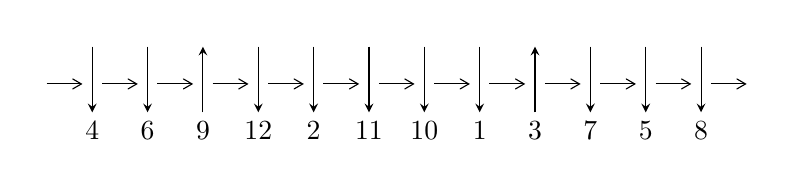
\begin{tikzpicture}[x=20pt, y=17pt]
	% nodes
	\node (C0) at (0, 0) {};
	\node (C1) at (1, 0) {};
	\node (C1U) at (1, +1) {};
	\node (C1D) at (1, -1) {4};

	\node (C2) at (2, 0) {};
	\node (C2U) at (2, +1) {};
	\node (C2D) at (2, -1) {6};

	\node (C3) at (3, 0) {};
	\node (C3U) at (3, +1) {};
	\node (C3D) at (3, -1) {9};

	\node (C4) at (4, 0) {};
	\node (C4U) at (4, +1) {};
	\node (C4D) at (4, -1) {12};

	\node (C5) at (5, 0) {};
	\node (C5U) at (5, +1) {};
	\node (C5D) at (5, -1) {2};

	\node (C6) at (6, 0) {};
	\node (C6U) at (6, +1) {};
	\node (C6D) at (6, -1) {11};

	\node (C7) at (7, 0) {};
	\node (C7U) at (7, +1) {};
	\node (C7D) at (7, -1) {10};

	\node (C8) at (8, 0) {};
	\node (C8U) at (8, +1) {};
	\node (C8D) at (8, -1) {1};

	\node (C9) at (9, 0) {};
	\node (C9U) at (9, +1) {};
	\node (C9D) at (9, -1) {3};

	\node (C10) at (10, 0) {};
	\node (C10U) at (10, +1) {};
	\node (C10D) at (10, -1) {7};

	\node (C11) at (11, 0) {};
	\node (C11U) at (11, +1) {};
	\node (C11D) at (11, -1) {5};

	\node (C12) at (12, 0) {};
	\node (C12U) at (12, +1) {};
	\node (C12D) at (12, -1) {8};
	\node (C13) at (13, 0) {};

	% arrows
	\draw[->,>={angle 60}]
	(C0) edge (C1) (C1) edge (C2) (C2) edge (C3) (C3) edge (C4) (C4) edge (C5) (C5) edge (C6) (C6) edge (C7) (C7) edge (C8) (C8) edge (C9) (C9) edge (C10) (C10) edge (C11) (C11) edge (C12) (C12) edge (C13) ;	\draw[->,>=stealth]
	(C1U) edge (C1D) (C2U) edge (C2D) (C3D) edge (C3U) (C4U) edge (C4D) (C5U) edge (C5D) (C6U) edge (C6D) (C7U) edge (C7D) (C8U) edge (C8D) (C9D) edge (C9U) (C10U) edge (C10D) (C11U) edge (C11D) (C12U) edge (C12D) ;
	\end{tikzpicture} \\
\hhline{~~} \\& 
\textbf{Solving Sequence} \\ \cline{2-2} 
 &
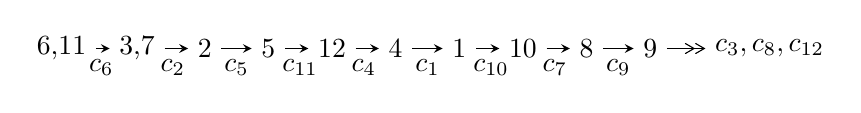
\begin{tikzpicture}[x=23pt, y=7pt]
	% node
	\node (A0) at (-1/8, 0) {6,11};
	\node (A1) at (17/16, 0) {3,7};
	\node (A2) at (17/8, 0) {2};
	\node (A3) at (25/8, 0) {5};
	\node (A4) at (33/8, 0) {12};
	\node (A5) at (41/8, 0) {4};
	\node (A6) at (49/8, 0) {1};
	\node (A7) at (57/8, 0) {10};
	\node (A8) at (65/8, 0) {8};
	\node (A9) at (73/8, 0) {9};
	\node (C1) at (1/2, -1) {$c_{6}$};
	\node (C2) at (13/8, -1) {$c_{2}$};
	\node (C3) at (21/8, -1) {$c_{5}$};
	\node (C4) at (29/8, -1) {$c_{11}$};
	\node (C5) at (37/8, -1) {$c_{4}$};
	\node (C6) at (45/8, -1) {$c_{1}$};
	\node (C7) at (53/8, -1) {$c_{10}$};
	\node (C8) at (61/8, -1) {$c_{7}$};
	\node (C9) at (69/8, -1) {$c_{9}$};
	\node (A10) at (11, 0) {$c_{3},c_{8},c_{12}$};

	% edge
	\draw[->,>=stealth]	
	(A0) edge (A1) (A1) edge (A2) (A2) edge (A3) (A3) edge (A4) (A4) edge (A5) (A5) edge (A6) (A6) edge (A7) (A7) edge (A8) (A8) edge (A9) ;
	\draw[->>,>={angle 60}]	
	(A9) edge (A10);
\end{tikzpicture} \\ 

\end{tabular} \\

\footnotetext{
The image of knot diagram is generated by the software ``\textbf{Draw programme}" developed by Andrew Bartholomew(\url{http://www.layer8.co.uk/maths/draw/index.htm\#Running-draw}), where we modified some parts for our purpose(\url{https://github.com/CATsTAILs/LinksPainter}).
}\phantom \\ \newline 
\centering \textbf{Ideals for irreducible components\footnotemark of $X_{\text{par}}$} 
 
\begin{align*}
I^u_{1}&=\langle 
1.48358\times10^{325} u^{114}-8.83956\times10^{325} u^{113}+\cdots+7.90184\times10^{326} b+4.90948\times10^{327},\\
\phantom{I^u_{1}}&\phantom{= \langle  }-3.66178\times10^{326} u^{114}+1.68734\times10^{327} u^{113}+\cdots+8.69202\times10^{327} a+1.06744\times10^{330},\\
\phantom{I^u_{1}}&\phantom{= \langle  }u^{115}-4 u^{114}+\cdots-3274 u-242\rangle \\
I^u_{2}&=\langle 
1493260 u^{25}-2702182 u^{24}+\cdots+2800453 b+235054,\\
\phantom{I^u_{2}}&\phantom{= \langle  }-5509815 u^{25}+13098661 u^{24}+\cdots+2800453 a+35107117,\;u^{26}-3 u^{25}+\cdots-4 u-1\rangle \\
\\
I^v_{1}&=\langle 
a,\;b+1,\;v-1\rangle \\
\end{align*}
\raggedright * 3 irreducible components of $\dim_{\mathbb{C}}=0$, with total 142 representations.\\
\footnotetext{All coefficients of polynomials are rational numbers. But the coefficients are sometimes approximated in decimal forms when there is not enough margin.}
\newpage
\renewcommand{\arraystretch}{1}
\centering \section*{I. $I^u_{1}= \langle 1.48\times10^{325} u^{114}-8.84\times10^{325} u^{113}+\cdots+7.90\times10^{326} b+4.91\times10^{327},\;-3.66\times10^{326} u^{114}+1.69\times10^{327} u^{113}+\cdots+8.69\times10^{327} a+1.07\times10^{330},\;u^{115}-4 u^{114}+\cdots-3274 u-242 \rangle$}
\flushleft \textbf{(i) Arc colorings}\\
\begin{tabular}{m{7pt} m{180pt} m{7pt} m{180pt} }
\flushright $a_{6}=$&$\begin{pmatrix}1\\0\end{pmatrix}$ \\
\flushright $a_{11}=$&$\begin{pmatrix}0\\u\end{pmatrix}$ \\
\flushright $a_{3}=$&$\begin{pmatrix}0.0421280 u^{114}-0.194125 u^{113}+\cdots+402.402 u-122.807\\-0.0187752 u^{114}+0.111867 u^{113}+\cdots-67.9999 u-6.21309\end{pmatrix}$ \\
\flushright $a_{7}=$&$\begin{pmatrix}1\\u^2\end{pmatrix}$ \\
\flushright $a_{2}=$&$\begin{pmatrix}0.0233528 u^{114}-0.0822580 u^{113}+\cdots+334.402 u-129.020\\-0.0187752 u^{114}+0.111867 u^{113}+\cdots-67.9999 u-6.21309\end{pmatrix}$ \\
\flushright $a_{5}=$&$\begin{pmatrix}0.0195044 u^{114}-0.0841949 u^{113}+\cdots+366.451 u-125.417\\0.00135440 u^{114}-0.0548362 u^{113}+\cdots+98.6890 u+6.28798\end{pmatrix}$ \\
\flushright $a_{12}=$&$\begin{pmatrix}-0.271850 u^{114}+1.10221 u^{113}+\cdots-3237.07 u+1136.06\\-0.0276167 u^{114}+0.116244 u^{113}+\cdots-35.5419 u+6.29003\end{pmatrix}$ \\
\flushright $a_{4}=$&$\begin{pmatrix}2.58291 u^{114}-10.5413 u^{113}+\cdots+29654.6 u-10368.4\\0.00832235 u^{114}-0.0902908 u^{113}+\cdots+304.045 u-61.6849\end{pmatrix}$ \\
\flushright $a_{1}=$&$\begin{pmatrix}-0.260596 u^{114}+1.06089 u^{113}+\cdots-3246.69 u+1136.50\\-0.0126304 u^{114}+0.0556980 u^{113}+\cdots-34.1711 u+6.56494\end{pmatrix}$ \\
\flushright $a_{10}=$&$\begin{pmatrix}u\\u^3+u\end{pmatrix}$ \\
\flushright $a_{8}=$&$\begin{pmatrix}u^2+1\\u^4+2 u^2\end{pmatrix}$ \\
\flushright $a_{9}=$&$\begin{pmatrix}-0.324366 u^{114}+1.30828 u^{113}+\cdots-3219.50 u+1138.13\\0.0181005 u^{114}-0.0871095 u^{113}+\cdots+9.95112 u+10.1619\end{pmatrix}$\\&\end{tabular}
\flushleft \textbf{(ii) Obstruction class $= -1$}\\~\\
\flushleft \textbf{(iii) Cusp Shapes $= 0.530416 u^{114}-2.22908 u^{113}+\cdots+5554.59 u-1891.64$}\\~\\
\newpage\renewcommand{\arraystretch}{1}
\flushleft \textbf{(iv) u-Polynomials at the component}\newline \\
\begin{tabular}{m{50pt}|m{274pt}}
Crossings & \hspace{64pt}u-Polynomials at each crossing \\
\hline $$\begin{aligned}c_{1}\end{aligned}$$&$\begin{aligned}
&u^{115}-2 u^{114}+\cdots-533977 u-135887
\end{aligned}$\\
\hline $$\begin{aligned}c_{2},c_{5}\end{aligned}$$&$\begin{aligned}
&u^{115}-29 u^{113}+\cdots+489 u-103
\end{aligned}$\\
\hline $$\begin{aligned}c_{3},c_{9}\end{aligned}$$&$\begin{aligned}
&u^{115}-14 u^{114}+\cdots-1475781 u-602561
\end{aligned}$\\
\hline $$\begin{aligned}c_{4},c_{11}\end{aligned}$$&$\begin{aligned}
&u^{115}-4 u^{114}+\cdots+5559 u-7129
\end{aligned}$\\
\hline $$\begin{aligned}c_{6},c_{7},c_{10}\end{aligned}$$&$\begin{aligned}
&u^{115}-4 u^{114}+\cdots-3274 u-242
\end{aligned}$\\
\hline $$\begin{aligned}c_{8},c_{12}\end{aligned}$$&$\begin{aligned}
&u^{115}-2 u^{114}+\cdots+5984 u+161
\end{aligned}$\\
\hline
\end{tabular}\\~\\
\newpage\renewcommand{\arraystretch}{1}
\flushleft \textbf{(v) Riley Polynomials at the component}\newline \\
\begin{tabular}{m{50pt}|m{274pt}}
Crossings & \hspace{64pt}Riley Polynomials at each crossing \\
\hline $$\begin{aligned}c_{1}\end{aligned}$$&$\begin{aligned}
&y^{115}-36 y^{114}+\cdots+2122072013805 y-18465276769
\end{aligned}$\\
\hline $$\begin{aligned}c_{2},c_{5}\end{aligned}$$&$\begin{aligned}
&y^{115}-58 y^{114}+\cdots+1346371 y-10609
\end{aligned}$\\
\hline $$\begin{aligned}c_{3},c_{9}\end{aligned}$$&$\begin{aligned}
&y^{115}-10 y^{114}+\cdots-1560457704043 y-363079758721
\end{aligned}$\\
\hline $$\begin{aligned}c_{4},c_{11}\end{aligned}$$&$\begin{aligned}
&y^{115}-18 y^{114}+\cdots-1151442169 y-50822641
\end{aligned}$\\
\hline $$\begin{aligned}c_{6},c_{7},c_{10}\end{aligned}$$&$\begin{aligned}
&y^{115}+110 y^{114}+\cdots+16205216 y-58564
\end{aligned}$\\
\hline $$\begin{aligned}c_{8},c_{12}\end{aligned}$$&$\begin{aligned}
&y^{115}-64 y^{114}+\cdots+53494106 y-25921
\end{aligned}$\\
\hline
\end{tabular}\\~\\
\newpage\flushleft \textbf{(vi) Complex Volumes and Cusp Shapes}
$$\begin{array}{c|c|c}  
\text{Solutions to }I^u_{1}& \I (\text{vol} + \sqrt{-1}CS) & \text{Cusp shape}\\
 \hline 
\begin{aligned}
u &= -0.848760 + 0.535653 I \\
a &= \phantom{-}0.353637 + 0.142381 I \\
b &= \phantom{-}0.863015 + 0.497078 I\end{aligned}
 & -1.40376 - 2.80497 I & \phantom{-0.000000 } 0 \\ \hline\begin{aligned}
u &= -0.848760 - 0.535653 I \\
a &= \phantom{-}0.353637 - 0.142381 I \\
b &= \phantom{-}0.863015 - 0.497078 I\end{aligned}
 & -1.40376 + 2.80497 I & \phantom{-0.000000 } 0 \\ \hline\begin{aligned}
u &= \phantom{-}0.444128 + 0.862264 I \\
a &= -0.490281 - 0.258396 I \\
b &= \phantom{-}1.42270 - 0.07493 I\end{aligned}
 & -8.31558 + 2.30847 I & \phantom{-0.000000 } 0 \\ \hline\begin{aligned}
u &= \phantom{-}0.444128 - 0.862264 I \\
a &= -0.490281 + 0.258396 I \\
b &= \phantom{-}1.42270 + 0.07493 I\end{aligned}
 & -8.31558 - 2.30847 I & \phantom{-0.000000 } 0 \\ \hline\begin{aligned}
u &= -0.871451 + 0.401674 I \\
a &= -0.356059 - 0.600521 I \\
b &= -1.244120 + 0.593087 I\end{aligned}
 & -2.05582 + 7.19848 I & \phantom{-0.000000 } 0 \\ \hline\begin{aligned}
u &= -0.871451 - 0.401674 I \\
a &= -0.356059 + 0.600521 I \\
b &= -1.244120 - 0.593087 I\end{aligned}
 & -2.05582 - 7.19848 I & \phantom{-0.000000 } 0 \\ \hline\begin{aligned}
u &= \phantom{-}0.806197 + 0.515754 I \\
a &= -1.230610 + 0.036542 I \\
b &= -0.725232 - 0.335010 I\end{aligned}
 & -2.92657 + 3.35414 I & \phantom{-0.000000 } 0 \\ \hline\begin{aligned}
u &= \phantom{-}0.806197 - 0.515754 I \\
a &= -1.230610 - 0.036542 I \\
b &= -0.725232 + 0.335010 I\end{aligned}
 & -2.92657 - 3.35414 I & \phantom{-0.000000 } 0 \\ \hline\begin{aligned}
u &= -0.942893 + 0.152410 I \\
a &= \phantom{-}0.722614 + 0.211941 I \\
b &= \phantom{-}0.842318 - 0.416431 I\end{aligned}
 & -1.27183 + 1.02449 I & \phantom{-0.000000 } 0 \\ \hline\begin{aligned}
u &= -0.942893 - 0.152410 I \\
a &= \phantom{-}0.722614 - 0.211941 I \\
b &= \phantom{-}0.842318 + 0.416431 I\end{aligned}
 & -1.27183 - 1.02449 I & \phantom{-0.000000 } 0\\
 \hline 
 \end{array}$$\newpage$$\begin{array}{c|c|c}  
\text{Solutions to }I^u_{1}& \I (\text{vol} + \sqrt{-1}CS) & \text{Cusp shape}\\
 \hline 
\begin{aligned}
u &= \phantom{-}1.055710 + 0.208614 I \\
a &= \phantom{-}0.535514 + 0.029917 I \\
b &= \phantom{-}0.831687 - 0.565650 I\end{aligned}
 & -0.09056 + 2.26730 I & \phantom{-0.000000 } 0 \\ \hline\begin{aligned}
u &= \phantom{-}1.055710 - 0.208614 I \\
a &= \phantom{-}0.535514 - 0.029917 I \\
b &= \phantom{-}0.831687 + 0.565650 I\end{aligned}
 & -0.09056 - 2.26730 I & \phantom{-0.000000 } 0 \\ \hline\begin{aligned}
u &= -0.819748 + 0.738480 I \\
a &= \phantom{-}0.325821 - 0.558599 I \\
b &= -1.017700 - 0.295821 I\end{aligned}
 & -1.06654 - 1.68639 I & \phantom{-0.000000 } 0 \\ \hline\begin{aligned}
u &= -0.819748 - 0.738480 I \\
a &= \phantom{-}0.325821 + 0.558599 I \\
b &= -1.017700 + 0.295821 I\end{aligned}
 & -1.06654 + 1.68639 I & \phantom{-0.000000 } 0 \\ \hline\begin{aligned}
u &= \phantom{-}1.035380 + 0.387132 I \\
a &= -0.397265 + 0.551227 I \\
b &= -1.213290 - 0.580536 I\end{aligned}
 & -5.7222 - 13.0581 I & \phantom{-0.000000 } 0 \\ \hline\begin{aligned}
u &= \phantom{-}1.035380 - 0.387132 I \\
a &= -0.397265 - 0.551227 I \\
b &= -1.213290 + 0.580536 I\end{aligned}
 & -5.7222 + 13.0581 I & \phantom{-0.000000 } 0 \\ \hline\begin{aligned}
u &= -0.720811 + 0.507644 I \\
a &= -0.007287 + 0.842062 I \\
b &= \phantom{-}1.261910 - 0.166931 I\end{aligned}
 & -5.37650 + 2.40064 I & \phantom{-0.000000 } 0 \\ \hline\begin{aligned}
u &= -0.720811 - 0.507644 I \\
a &= -0.007287 - 0.842062 I \\
b &= \phantom{-}1.261910 + 0.166931 I\end{aligned}
 & -5.37650 - 2.40064 I & \phantom{-0.000000 } 0 \\ \hline\begin{aligned}
u &= \phantom{-}0.792446 + 0.355091 I \\
a &= \phantom{-}0.287125 - 1.113030 I \\
b &= \phantom{-}1.267030 + 0.275005 I\end{aligned}
 & -9.78230 - 6.84107 I & \phantom{-0.000000 } 0 \\ \hline\begin{aligned}
u &= \phantom{-}0.792446 - 0.355091 I \\
a &= \phantom{-}0.287125 + 1.113030 I \\
b &= \phantom{-}1.267030 - 0.275005 I\end{aligned}
 & -9.78230 + 6.84107 I & \phantom{-0.000000 } 0\\
 \hline 
 \end{array}$$\newpage$$\begin{array}{c|c|c}  
\text{Solutions to }I^u_{1}& \I (\text{vol} + \sqrt{-1}CS) & \text{Cusp shape}\\
 \hline 
\begin{aligned}
u &= -0.007272 + 1.137120 I \\
a &= -0.01929 + 2.37332 I \\
b &= \phantom{-}0.785173 - 0.793722 I\end{aligned}
 & -1.08900 + 5.90884 I & \phantom{-0.000000 } 0 \\ \hline\begin{aligned}
u &= -0.007272 - 1.137120 I \\
a &= -0.01929 - 2.37332 I \\
b &= \phantom{-}0.785173 + 0.793722 I\end{aligned}
 & -1.08900 - 5.90884 I & \phantom{-0.000000 } 0 \\ \hline\begin{aligned}
u &= -0.444865 + 0.728686 I \\
a &= -0.128324 - 0.238843 I \\
b &= \phantom{-}0.287556 + 0.640106 I\end{aligned}
 & \phantom{-}1.04492 + 3.26813 I & \phantom{-0.000000 } 0 \\ \hline\begin{aligned}
u &= -0.444865 - 0.728686 I \\
a &= -0.128324 + 0.238843 I \\
b &= \phantom{-}0.287556 - 0.640106 I\end{aligned}
 & \phantom{-}1.04492 - 3.26813 I & \phantom{-0.000000 } 0 \\ \hline\begin{aligned}
u &= -0.667184 + 0.506083 I \\
a &= \phantom{-}1.08713 + 0.90478 I \\
b &= \phantom{-}1.072640 - 0.507155 I\end{aligned}
 & -1.13029 + 7.69736 I & \phantom{-0.000000 } 0 \\ \hline\begin{aligned}
u &= -0.667184 - 0.506083 I \\
a &= \phantom{-}1.08713 - 0.90478 I \\
b &= \phantom{-}1.072640 + 0.507155 I\end{aligned}
 & -1.13029 - 7.69736 I & \phantom{-0.000000 } 0 \\ \hline\begin{aligned}
u &= \phantom{-}0.133758 + 1.163830 I \\
a &= \phantom{-}0.90734 - 1.40822 I \\
b &= -0.726636 + 0.740712 I\end{aligned}
 & -1.92843 + 0.18544 I & \phantom{-0.000000 } 0 \\ \hline\begin{aligned}
u &= \phantom{-}0.133758 - 1.163830 I \\
a &= \phantom{-}0.90734 + 1.40822 I \\
b &= -0.726636 - 0.740712 I\end{aligned}
 & -1.92843 - 0.18544 I & \phantom{-0.000000 } 0 \\ \hline\begin{aligned}
u &= -0.820611 + 0.022404 I \\
a &= -0.831148 + 0.746544 I \\
b &= -0.871734 + 0.225452 I\end{aligned}
 & -0.420463 + 0.454049 I & \phantom{-0.000000 } 0 \\ \hline\begin{aligned}
u &= -0.820611 - 0.022404 I \\
a &= -0.831148 - 0.746544 I \\
b &= -0.871734 - 0.225452 I\end{aligned}
 & -0.420463 - 0.454049 I & \phantom{-0.000000 } 0\\
 \hline 
 \end{array}$$\newpage$$\begin{array}{c|c|c}  
\text{Solutions to }I^u_{1}& \I (\text{vol} + \sqrt{-1}CS) & \text{Cusp shape}\\
 \hline 
\begin{aligned}
u &= \phantom{-}0.342572 + 1.132270 I \\
a &= \phantom{-}1.027390 - 0.110480 I \\
b &= -1.309470 + 0.407989 I\end{aligned}
 & -4.24872 - 2.09284 I & \phantom{-0.000000 } 0 \\ \hline\begin{aligned}
u &= \phantom{-}0.342572 - 1.132270 I \\
a &= \phantom{-}1.027390 + 0.110480 I \\
b &= -1.309470 - 0.407989 I\end{aligned}
 & -4.24872 + 2.09284 I & \phantom{-0.000000 } 0 \\ \hline\begin{aligned}
u &= \phantom{-}0.164195 + 1.186280 I \\
a &= -0.39920 + 1.92337 I \\
b &= \phantom{-}0.335099 - 0.255524 I\end{aligned}
 & -1.21977 - 6.97522 I & \phantom{-0.000000 } 0 \\ \hline\begin{aligned}
u &= \phantom{-}0.164195 - 1.186280 I \\
a &= -0.39920 - 1.92337 I \\
b &= \phantom{-}0.335099 + 0.255524 I\end{aligned}
 & -1.21977 + 6.97522 I & \phantom{-0.000000 } 0 \\ \hline\begin{aligned}
u &= \phantom{-}0.777862 + 0.126290 I \\
a &= -0.460508 + 0.703488 I \\
b &= -1.170850 - 0.640764 I\end{aligned}
 & -7.30108 - 1.98752 I & \phantom{-0.000000 } 0 \\ \hline\begin{aligned}
u &= \phantom{-}0.777862 - 0.126290 I \\
a &= -0.460508 - 0.703488 I \\
b &= -1.170850 + 0.640764 I\end{aligned}
 & -7.30108 + 1.98752 I & \phantom{-0.000000 } 0 \\ \hline\begin{aligned}
u &= -0.024539 + 1.266100 I \\
a &= \phantom{-}0.262122 - 1.308580 I \\
b &= \phantom{-}0.366022 + 0.297777 I\end{aligned}
 & \phantom{-}3.90810 + 2.10519 I & \phantom{-0.000000 } 0 \\ \hline\begin{aligned}
u &= -0.024539 - 1.266100 I \\
a &= \phantom{-}0.262122 + 1.308580 I \\
b &= \phantom{-}0.366022 - 0.297777 I\end{aligned}
 & \phantom{-}3.90810 - 2.10519 I & \phantom{-0.000000 } 0 \\ \hline\begin{aligned}
u &= -0.114979 + 1.264060 I \\
a &= -0.19552 - 2.44022 I \\
b &= \phantom{-}0.183040 + 1.265380 I\end{aligned}
 & \phantom{-}4.64254 + 0.78526 I & \phantom{-0.000000 } 0 \\ \hline\begin{aligned}
u &= -0.114979 - 1.264060 I \\
a &= -0.19552 + 2.44022 I \\
b &= \phantom{-}0.183040 - 1.265380 I\end{aligned}
 & \phantom{-}4.64254 - 0.78526 I & \phantom{-0.000000 } 0\\
 \hline 
 \end{array}$$\newpage$$\begin{array}{c|c|c}  
\text{Solutions to }I^u_{1}& \I (\text{vol} + \sqrt{-1}CS) & \text{Cusp shape}\\
 \hline 
\begin{aligned}
u &= \phantom{-}0.593045 + 0.396313 I \\
a &= -0.705193 - 0.411959 I \\
b &= -0.148133 + 0.960454 I\end{aligned}
 & -2.59156 - 7.60766 I & -8.00000 + 6.69285 I \\ \hline\begin{aligned}
u &= \phantom{-}0.593045 - 0.396313 I \\
a &= -0.705193 + 0.411959 I \\
b &= -0.148133 - 0.960454 I\end{aligned}
 & -2.59156 + 7.60766 I & -8.00000 - 6.69285 I \\ \hline\begin{aligned}
u &= \phantom{-}0.051284 + 1.291940 I \\
a &= -1.130690 + 0.261646 I \\
b &= \phantom{-}1.98739 - 0.20444 I\end{aligned}
 & -4.87527 - 3.60685 I & \phantom{-0.000000 } 0 \\ \hline\begin{aligned}
u &= \phantom{-}0.051284 - 1.291940 I \\
a &= -1.130690 - 0.261646 I \\
b &= \phantom{-}1.98739 + 0.20444 I\end{aligned}
 & -4.87527 + 3.60685 I & \phantom{-0.000000 } 0 \\ \hline\begin{aligned}
u &= -0.319473 + 1.257690 I \\
a &= \phantom{-}0.242862 + 0.596086 I \\
b &= \phantom{-}0.669671 - 0.148467 I\end{aligned}
 & \phantom{-}2.10936 + 3.26957 I & \phantom{-0.000000 } 0 \\ \hline\begin{aligned}
u &= -0.319473 - 1.257690 I \\
a &= \phantom{-}0.242862 - 0.596086 I \\
b &= \phantom{-}0.669671 + 0.148467 I\end{aligned}
 & \phantom{-}2.10936 - 3.26957 I & \phantom{-0.000000 } 0 \\ \hline\begin{aligned}
u &= \phantom{-}0.689850 + 0.076744 I \\
a &= -0.307075 + 0.730969 I \\
b &= -0.290572 - 0.773586 I\end{aligned}
 & -4.99291 - 3.33304 I & -13.08615 + 3.39546 I \\ \hline\begin{aligned}
u &= \phantom{-}0.689850 - 0.076744 I \\
a &= -0.307075 - 0.730969 I \\
b &= -0.290572 + 0.773586 I\end{aligned}
 & -4.99291 + 3.33304 I & -13.08615 - 3.39546 I \\ \hline\begin{aligned}
u &= -0.023304 + 1.306530 I \\
a &= -0.59051 - 1.33130 I \\
b &= -1.185790 + 0.271332 I\end{aligned}
 & \phantom{-}0.569428 + 0.425875 I & \phantom{-0.000000 } 0 \\ \hline\begin{aligned}
u &= -0.023304 - 1.306530 I \\
a &= -0.59051 + 1.33130 I \\
b &= -1.185790 - 0.271332 I\end{aligned}
 & \phantom{-}0.569428 - 0.425875 I & \phantom{-0.000000 } 0\\
 \hline 
 \end{array}$$\newpage$$\begin{array}{c|c|c}  
\text{Solutions to }I^u_{1}& \I (\text{vol} + \sqrt{-1}CS) & \text{Cusp shape}\\
 \hline 
\begin{aligned}
u &= \phantom{-}0.334393 + 1.265360 I \\
a &= -0.47433 + 1.62982 I \\
b &= -0.312042 - 0.651579 I\end{aligned}
 & -0.88935 - 7.00364 I & \phantom{-0.000000 } 0 \\ \hline\begin{aligned}
u &= \phantom{-}0.334393 - 1.265360 I \\
a &= -0.47433 - 1.62982 I \\
b &= -0.312042 + 0.651579 I\end{aligned}
 & -0.88935 + 7.00364 I & \phantom{-0.000000 } 0 \\ \hline\begin{aligned}
u &= \phantom{-}0.145936 + 0.646760 I \\
a &= \phantom{-}1.93330 - 0.69519 I \\
b &= -0.431275 + 0.236192 I\end{aligned}
 & -2.29797 + 0.41180 I & -6.91359 + 0. I\phantom{ +0.000000I} \\ \hline\begin{aligned}
u &= \phantom{-}0.145936 - 0.646760 I \\
a &= \phantom{-}1.93330 + 0.69519 I \\
b &= -0.431275 - 0.236192 I\end{aligned}
 & -2.29797 - 0.41180 I & -6.91359 + 0. I\phantom{ +0.000000I} \\ \hline\begin{aligned}
u &= \phantom{-}0.045172 + 1.348770 I \\
a &= \phantom{-}0.35576 + 1.44895 I \\
b &= -1.025840 - 0.495040 I\end{aligned}
 & \phantom{-}2.73002 - 1.02745 I & \phantom{-0.000000 } 0 \\ \hline\begin{aligned}
u &= \phantom{-}0.045172 - 1.348770 I \\
a &= \phantom{-}0.35576 - 1.44895 I \\
b &= -1.025840 + 0.495040 I\end{aligned}
 & \phantom{-}2.73002 + 1.02745 I & \phantom{-0.000000 } 0 \\ \hline\begin{aligned}
u &= \phantom{-}0.244481 + 0.581940 I \\
a &= -0.337020 - 0.312300 I \\
b &= \phantom{-}0.523607 - 0.703589 I\end{aligned}
 & \phantom{-}3.31672 + 1.01238 I & \phantom{-0.000000 } 0. - 2.79142 I \\ \hline\begin{aligned}
u &= \phantom{-}0.244481 - 0.581940 I \\
a &= -0.337020 + 0.312300 I \\
b &= \phantom{-}0.523607 + 0.703589 I\end{aligned}
 & \phantom{-}3.31672 - 1.01238 I & \phantom{-0.000000 -}0. + 2.79142 I \\ \hline\begin{aligned}
u &= \phantom{-}0.317987 + 1.350110 I \\
a &= \phantom{-}0.30106 + 1.88497 I \\
b &= -1.052110 - 0.853041 I\end{aligned}
 & -2.64224 - 5.93833 I & \phantom{-0.000000 } 0 \\ \hline\begin{aligned}
u &= \phantom{-}0.317987 - 1.350110 I \\
a &= \phantom{-}0.30106 - 1.88497 I \\
b &= -1.052110 + 0.853041 I\end{aligned}
 & -2.64224 + 5.93833 I & \phantom{-0.000000 } 0\\
 \hline 
 \end{array}$$\newpage$$\begin{array}{c|c|c}  
\text{Solutions to }I^u_{1}& \I (\text{vol} + \sqrt{-1}CS) & \text{Cusp shape}\\
 \hline 
\begin{aligned}
u &= \phantom{-}0.905787 + 1.055960 I \\
a &= \phantom{-}0.308652 + 0.202276 I \\
b &= -0.998116 + 0.396976 I\end{aligned}
 & -3.92358 + 6.50991 I & \phantom{-0.000000 } 0 \\ \hline\begin{aligned}
u &= \phantom{-}0.905787 - 1.055960 I \\
a &= \phantom{-}0.308652 - 0.202276 I \\
b &= -0.998116 - 0.396976 I\end{aligned}
 & -3.92358 - 6.50991 I & \phantom{-0.000000 } 0 \\ \hline\begin{aligned}
u &= -0.203376 + 1.378930 I \\
a &= \phantom{-}0.32768 - 1.41692 I \\
b &= -0.606279 + 0.411879 I\end{aligned}
 & \phantom{-}4.08974 + 2.88264 I & \phantom{-0.000000 } 0 \\ \hline\begin{aligned}
u &= -0.203376 - 1.378930 I \\
a &= \phantom{-}0.32768 + 1.41692 I \\
b &= -0.606279 - 0.411879 I\end{aligned}
 & \phantom{-}4.08974 - 2.88264 I & \phantom{-0.000000 } 0 \\ \hline\begin{aligned}
u &= \phantom{-}0.543376 + 0.245663 I \\
a &= \phantom{-}1.50482 - 0.35020 I \\
b &= \phantom{-}0.995267 + 0.546016 I\end{aligned}
 & \phantom{-}1.94742 - 3.73444 I & -2.99201 + 4.54253 I \\ \hline\begin{aligned}
u &= \phantom{-}0.543376 - 0.245663 I \\
a &= \phantom{-}1.50482 + 0.35020 I \\
b &= \phantom{-}0.995267 - 0.546016 I\end{aligned}
 & \phantom{-}1.94742 + 3.73444 I & -2.99201 - 4.54253 I \\ \hline\begin{aligned}
u &= -0.180518 + 1.393110 I \\
a &= \phantom{-}0.71276 + 1.65856 I \\
b &= -0.69614 - 1.51255 I\end{aligned}
 & \phantom{-}6.32602 + 3.38126 I & \phantom{-0.000000 } 0 \\ \hline\begin{aligned}
u &= -0.180518 - 1.393110 I \\
a &= \phantom{-}0.71276 - 1.65856 I \\
b &= -0.69614 + 1.51255 I\end{aligned}
 & \phantom{-}6.32602 - 3.38126 I & \phantom{-0.000000 } 0 \\ \hline\begin{aligned}
u &= \phantom{-}0.052810 + 1.408130 I \\
a &= \phantom{-}0.95246 + 2.48551 I \\
b &= -0.919359 - 0.186590 I\end{aligned}
 & \phantom{-}1.73762 - 0.50100 I & \phantom{-0.000000 } 0 \\ \hline\begin{aligned}
u &= \phantom{-}0.052810 - 1.408130 I \\
a &= \phantom{-}0.95246 - 2.48551 I \\
b &= -0.919359 + 0.186590 I\end{aligned}
 & \phantom{-}1.73762 + 0.50100 I & \phantom{-0.000000 } 0\\
 \hline 
 \end{array}$$\newpage$$\begin{array}{c|c|c}  
\text{Solutions to }I^u_{1}& \I (\text{vol} + \sqrt{-1}CS) & \text{Cusp shape}\\
 \hline 
\begin{aligned}
u &= \phantom{-}0.20254 + 1.40986 I \\
a &= -0.15648 - 1.53021 I \\
b &= \phantom{-}1.26724 + 0.71966 I\end{aligned}
 & \phantom{-}7.29078 - 6.44881 I & \phantom{-0.000000 } 0 \\ \hline\begin{aligned}
u &= \phantom{-}0.20254 - 1.40986 I \\
a &= -0.15648 + 1.53021 I \\
b &= \phantom{-}1.26724 - 0.71966 I\end{aligned}
 & \phantom{-}7.29078 + 6.44881 I & \phantom{-0.000000 } 0 \\ \hline\begin{aligned}
u &= \phantom{-}0.20423 + 1.43550 I \\
a &= -1.04385 - 1.28519 I \\
b &= \phantom{-}1.095920 + 0.612241 I\end{aligned}
 & -2.32289 + 0.32997 I & \phantom{-0.000000 } 0 \\ \hline\begin{aligned}
u &= \phantom{-}0.20423 - 1.43550 I \\
a &= -1.04385 + 1.28519 I \\
b &= \phantom{-}1.095920 - 0.612241 I\end{aligned}
 & -2.32289 - 0.32997 I & \phantom{-0.000000 } 0 \\ \hline\begin{aligned}
u &= -0.31362 + 1.42263 I \\
a &= \phantom{-}0.060785 - 0.787387 I \\
b &= -1.318410 + 0.422599 I\end{aligned}
 & \phantom{-}4.49338 + 4.70011 I & \phantom{-0.000000 } 0 \\ \hline\begin{aligned}
u &= -0.31362 - 1.42263 I \\
a &= \phantom{-}0.060785 + 0.787387 I \\
b &= -1.318410 - 0.422599 I\end{aligned}
 & \phantom{-}4.49338 - 4.70011 I & \phantom{-0.000000 } 0 \\ \hline\begin{aligned}
u &= \phantom{-}0.51530 + 1.37670 I \\
a &= \phantom{-}0.205635 - 1.272950 I \\
b &= \phantom{-}1.123530 + 0.658322 I\end{aligned}
 & \phantom{-}3.75436 - 8.01338 I & \phantom{-0.000000 } 0 \\ \hline\begin{aligned}
u &= \phantom{-}0.51530 - 1.37670 I \\
a &= \phantom{-}0.205635 + 1.272950 I \\
b &= \phantom{-}1.123530 - 0.658322 I\end{aligned}
 & \phantom{-}3.75436 + 8.01338 I & \phantom{-0.000000 } 0 \\ \hline\begin{aligned}
u &= \phantom{-}0.24043 + 1.45063 I \\
a &= \phantom{-}0.47198 - 1.47656 I \\
b &= -0.39633 + 1.38876 I\end{aligned}
 & \phantom{-}3.33246 - 10.74300 I & \phantom{-0.000000 } 0 \\ \hline\begin{aligned}
u &= \phantom{-}0.24043 - 1.45063 I \\
a &= \phantom{-}0.47198 + 1.47656 I \\
b &= -0.39633 - 1.38876 I\end{aligned}
 & \phantom{-}3.33246 + 10.74300 I & \phantom{-0.000000 } 0\\
 \hline 
 \end{array}$$\newpage$$\begin{array}{c|c|c}  
\text{Solutions to }I^u_{1}& \I (\text{vol} + \sqrt{-1}CS) & \text{Cusp shape}\\
 \hline 
\begin{aligned}
u &= -0.273683 + 0.449521 I \\
a &= -0.935505 + 0.381660 I \\
b &= -1.143250 - 0.176030 I\end{aligned}
 & -3.24070 + 0.76614 I & -9.29153 - 9.11952 I \\ \hline\begin{aligned}
u &= -0.273683 - 0.449521 I \\
a &= -0.935505 - 0.381660 I \\
b &= -1.143250 + 0.176030 I\end{aligned}
 & -3.24070 - 0.76614 I & -9.29153 + 9.11952 I \\ \hline\begin{aligned}
u &= -0.512024\phantom{ +0.000000I} \\
a &= \phantom{-}1.00918\phantom{ +0.000000I} \\
b &= \phantom{-}0.104589\phantom{ +0.000000I}\end{aligned}
 & -1.30525\phantom{ +0.000000I} & -8.04660\phantom{ +0.000000I} \\ \hline\begin{aligned}
u &= \phantom{-}0.03133 + 1.48977 I \\
a &= -0.463963 + 1.224590 I \\
b &= \phantom{-}0.375218 - 1.123290 I\end{aligned}
 & \phantom{-}10.10420 + 0.16194 I & \phantom{-0.000000 } 0 \\ \hline\begin{aligned}
u &= \phantom{-}0.03133 - 1.48977 I \\
a &= -0.463963 - 1.224590 I \\
b &= \phantom{-}0.375218 + 1.123290 I\end{aligned}
 & \phantom{-}10.10420 - 0.16194 I & \phantom{-0.000000 } 0 \\ \hline\begin{aligned}
u &= \phantom{-}0.30669 + 1.46839 I \\
a &= -0.59841 - 1.56983 I \\
b &= \phantom{-}1.141790 + 0.484176 I\end{aligned}
 & -3.90285 - 10.84020 I & \phantom{-0.000000 } 0 \\ \hline\begin{aligned}
u &= \phantom{-}0.30669 - 1.46839 I \\
a &= -0.59841 + 1.56983 I \\
b &= \phantom{-}1.141790 - 0.484176 I\end{aligned}
 & -3.90285 + 10.84020 I & \phantom{-0.000000 } 0 \\ \hline\begin{aligned}
u &= \phantom{-}0.15757 + 1.50056 I \\
a &= \phantom{-}0.194740 + 0.937959 I \\
b &= -1.282560 - 0.508335 I\end{aligned}
 & \phantom{-}4.20019 + 0.23370 I & \phantom{-0.000000 } 0 \\ \hline\begin{aligned}
u &= \phantom{-}0.15757 - 1.50056 I \\
a &= \phantom{-}0.194740 - 0.937959 I \\
b &= -1.282560 + 0.508335 I\end{aligned}
 & \phantom{-}4.20019 - 0.23370 I & \phantom{-0.000000 } 0 \\ \hline\begin{aligned}
u &= \phantom{-}0.28656 + 1.48163 I \\
a &= -0.294558 + 0.764011 I \\
b &= \phantom{-}0.441979 - 0.853938 I\end{aligned}
 & \phantom{-}5.78605 - 2.39116 I & \phantom{-0.000000 } 0\\
 \hline 
 \end{array}$$\newpage$$\begin{array}{c|c|c}  
\text{Solutions to }I^u_{1}& \I (\text{vol} + \sqrt{-1}CS) & \text{Cusp shape}\\
 \hline 
\begin{aligned}
u &= \phantom{-}0.28656 - 1.48163 I \\
a &= -0.294558 - 0.764011 I \\
b &= \phantom{-}0.441979 + 0.853938 I\end{aligned}
 & \phantom{-}5.78605 + 2.39116 I & \phantom{-0.000000 } 0 \\ \hline\begin{aligned}
u &= -0.24773 + 1.48985 I \\
a &= -0.12180 + 1.44164 I \\
b &= \phantom{-}1.28492 - 0.61531 I\end{aligned}
 & \phantom{-}5.28274 + 11.06650 I & \phantom{-0.000000 } 0 \\ \hline\begin{aligned}
u &= -0.24773 - 1.48985 I \\
a &= -0.12180 - 1.44164 I \\
b &= \phantom{-}1.28492 + 0.61531 I\end{aligned}
 & \phantom{-}5.28274 - 11.06650 I & \phantom{-0.000000 } 0 \\ \hline\begin{aligned}
u &= -0.26170 + 1.49467 I \\
a &= -0.70622 + 1.26852 I \\
b &= \phantom{-}1.152730 - 0.515773 I\end{aligned}
 & \phantom{-}1.09564 + 5.97831 I & \phantom{-0.000000 } 0 \\ \hline\begin{aligned}
u &= -0.26170 - 1.49467 I \\
a &= -0.70622 - 1.26852 I \\
b &= \phantom{-}1.152730 + 0.515773 I\end{aligned}
 & \phantom{-}1.09564 - 5.97831 I & \phantom{-0.000000 } 0 \\ \hline\begin{aligned}
u &= -0.33901 + 1.48133 I \\
a &= \phantom{-}0.38955 - 1.62191 I \\
b &= -1.31688 + 0.86138 I\end{aligned}
 & \phantom{-}3.96448 + 11.58650 I & \phantom{-0.000000 } 0 \\ \hline\begin{aligned}
u &= -0.33901 - 1.48133 I \\
a &= \phantom{-}0.38955 + 1.62191 I \\
b &= -1.31688 - 0.86138 I\end{aligned}
 & \phantom{-}3.96448 - 11.58650 I & \phantom{-0.000000 } 0 \\ \hline\begin{aligned}
u &= -0.436400 + 0.169728 I \\
a &= -0.859975 + 0.810724 I \\
b &= -0.319600 - 1.234530 I\end{aligned}
 & \phantom{-}1.21839 + 1.05065 I & -12.05031 - 7.14943 I \\ \hline\begin{aligned}
u &= -0.436400 - 0.169728 I \\
a &= -0.859975 - 0.810724 I \\
b &= -0.319600 + 1.234530 I\end{aligned}
 & \phantom{-}1.21839 - 1.05065 I & -12.05031 + 7.14943 I \\ \hline\begin{aligned}
u &= \phantom{-}0.313163 + 0.334163 I \\
a &= -1.21707 - 1.40078 I \\
b &= \phantom{-}1.53200 + 0.23250 I\end{aligned}
 & -8.16318 + 2.66336 I & -17.8732 - 3.5049 I\\
 \hline 
 \end{array}$$\newpage$$\begin{array}{c|c|c}  
\text{Solutions to }I^u_{1}& \I (\text{vol} + \sqrt{-1}CS) & \text{Cusp shape}\\
 \hline 
\begin{aligned}
u &= \phantom{-}0.313163 - 0.334163 I \\
a &= -1.21707 + 1.40078 I \\
b &= \phantom{-}1.53200 - 0.23250 I\end{aligned}
 & -8.16318 - 2.66336 I & -17.8732 + 3.5049 I \\ \hline\begin{aligned}
u &= -0.40800 + 1.49585 I \\
a &= -0.015891 + 1.219100 I \\
b &= \phantom{-}1.114320 - 0.615250 I\end{aligned}
 & \phantom{-}4.09278 + 6.12627 I & \phantom{-0.000000 } 0 \\ \hline\begin{aligned}
u &= -0.40800 - 1.49585 I \\
a &= -0.015891 - 1.219100 I \\
b &= \phantom{-}1.114320 + 0.615250 I\end{aligned}
 & \phantom{-}4.09278 - 6.12627 I & \phantom{-0.000000 } 0 \\ \hline\begin{aligned}
u &= -0.09800 + 1.55477 I \\
a &= -0.303147 - 1.145330 I \\
b &= \phantom{-}0.176377 + 1.012480 I\end{aligned}
 & \phantom{-}8.66726 + 5.18238 I & \phantom{-0.000000 } 0 \\ \hline\begin{aligned}
u &= -0.09800 - 1.55477 I \\
a &= -0.303147 + 1.145330 I \\
b &= \phantom{-}0.176377 - 1.012480 I\end{aligned}
 & \phantom{-}8.66726 - 5.18238 I & \phantom{-0.000000 } 0 \\ \hline\begin{aligned}
u &= \phantom{-}0.39745 + 1.50772 I \\
a &= \phantom{-}0.25992 + 1.54249 I \\
b &= -1.32257 - 0.77450 I\end{aligned}
 & \phantom{-}0.3285 - 18.1859 I & \phantom{-0.000000 } 0 \\ \hline\begin{aligned}
u &= \phantom{-}0.39745 - 1.50772 I \\
a &= \phantom{-}0.25992 - 1.54249 I \\
b &= -1.32257 + 0.77450 I\end{aligned}
 & \phantom{-}0.3285 + 18.1859 I & \phantom{-0.000000 } 0 \\ \hline\begin{aligned}
u &= -0.16909 + 1.55843 I \\
a &= -0.197722 - 0.873637 I \\
b &= \phantom{-}0.455786 + 0.780270 I\end{aligned}
 & \phantom{-}6.08178 + 0.84106 I & \phantom{-0.000000 } 0 \\ \hline\begin{aligned}
u &= -0.16909 - 1.55843 I \\
a &= -0.197722 + 0.873637 I \\
b &= \phantom{-}0.455786 - 0.780270 I\end{aligned}
 & \phantom{-}6.08178 - 0.84106 I & \phantom{-0.000000 } 0 \\ \hline\begin{aligned}
u &= -0.306547 + 0.215113 I \\
a &= \phantom{-}0.613994 - 1.264500 I \\
b &= -0.273298 + 0.261391 I\end{aligned}
 & -0.466771 + 0.832441 I & -9.34306 - 8.18046 I\\
 \hline 
 \end{array}$$\newpage$$\begin{array}{c|c|c}  
\text{Solutions to }I^u_{1}& \I (\text{vol} + \sqrt{-1}CS) & \text{Cusp shape}\\
 \hline 
\begin{aligned}
u &= -0.306547 - 0.215113 I \\
a &= \phantom{-}0.613994 + 1.264500 I \\
b &= -0.273298 - 0.261391 I\end{aligned}
 & -0.466771 - 0.832441 I & -9.34306 + 8.18046 I \\ \hline\begin{aligned}
u &= \phantom{-}0.295478\phantom{ +0.000000I} \\
a &= -2.56557\phantom{ +0.000000I} \\
b &= -0.923726\phantom{ +0.000000I}\end{aligned}
 & -1.51120\phantom{ +0.000000I} & -6.11550\phantom{ +0.000000I} \\ \hline\begin{aligned}
u &= -0.12927 + 1.83070 I \\
a &= \phantom{-}0.436548 - 0.143195 I \\
b &= -0.629747 - 0.003385 I\end{aligned}
 & \phantom{-}8.11054 + 2.74940 I & \phantom{-0.000000 } 0 \\ \hline\begin{aligned}
u &= -0.12927 - 1.83070 I \\
a &= \phantom{-}0.436548 + 0.143195 I \\
b &= -0.629747 + 0.003385 I\end{aligned}
 & \phantom{-}8.11054 - 2.74940 I & \phantom{-0.000000 } 0 \\ \hline\begin{aligned}
u &= -0.0610581\phantom{ +0.000000I} \\
a &= -148.073\phantom{ +0.000000I} \\
b &= -0.998011\phantom{ +0.000000I}\end{aligned}
 & -3.28783\phantom{ +0.000000I} & -2233.10\phantom{ +0.000000I}\\
 \hline 
 \end{array}$$\newpage\newpage\renewcommand{\arraystretch}{1}
\centering \section*{II. $I^u_{2}= \langle 1.49\times10^{6} u^{25}-2.70\times10^{6} u^{24}+\cdots+2.80\times10^{6} b+2.35\times10^{5},\;-5.51\times10^{6} u^{25}+1.31\times10^{7} u^{24}+\cdots+2.80\times10^{6} a+3.51\times10^{7},\;u^{26}-3 u^{25}+\cdots-4 u-1 \rangle$}
\flushleft \textbf{(i) Arc colorings}\\
\begin{tabular}{m{7pt} m{180pt} m{7pt} m{180pt} }
\flushright $a_{6}=$&$\begin{pmatrix}1\\0\end{pmatrix}$ \\
\flushright $a_{11}=$&$\begin{pmatrix}0\\u\end{pmatrix}$ \\
\flushright $a_{3}=$&$\begin{pmatrix}1.96747 u^{25}-4.67734 u^{24}+\cdots+69.2022 u-12.5362\\-0.533221 u^{25}+0.964909 u^{24}+\cdots+4.51107 u-0.0839343\end{pmatrix}$ \\
\flushright $a_{7}=$&$\begin{pmatrix}1\\u^2\end{pmatrix}$ \\
\flushright $a_{2}=$&$\begin{pmatrix}1.43425 u^{25}-3.71243 u^{24}+\cdots+73.7132 u-12.6202\\-0.533221 u^{25}+0.964909 u^{24}+\cdots+4.51107 u-0.0839343\end{pmatrix}$ \\
\flushright $a_{5}=$&$\begin{pmatrix}0.853886 u^{25}-2.98215 u^{24}+\cdots+72.8784 u-11.4277\\2.16059 u^{25}-6.83795 u^{24}+\cdots+4.43665 u+0.140403\end{pmatrix}$ \\
\flushright $a_{12}=$&$\begin{pmatrix}-3.03930 u^{25}+9.78221 u^{24}+\cdots-156.953 u+30.0998\\-0.202790 u^{25}+0.516128 u^{24}+\cdots-5.94755 u+1.34461\end{pmatrix}$ \\
\flushright $a_{4}=$&$\begin{pmatrix}9.15386 u^{25}-29.2824 u^{24}+\cdots+455.749 u-82.0067\\1.35608 u^{25}-3.57950 u^{24}+\cdots+17.4512 u-3.41836\end{pmatrix}$ \\
\flushright $a_{1}=$&$\begin{pmatrix}-3.37500 u^{25}+11.3334 u^{24}+\cdots-155.010 u+29.0605\\-0.261930 u^{25}+0.671359 u^{24}+\cdots-5.99244 u+1.39090\end{pmatrix}$ \\
\flushright $a_{10}=$&$\begin{pmatrix}u\\u^3+u\end{pmatrix}$ \\
\flushright $a_{8}=$&$\begin{pmatrix}u^2+1\\u^4+2 u^2\end{pmatrix}$ \\
\flushright $a_{9}=$&$\begin{pmatrix}-3.66510 u^{25}+10.1431 u^{24}+\cdots-158.439 u+30.4760\\0.200453 u^{25}+0.666037 u^{24}+\cdots-12.2579 u-0.121281\end{pmatrix}$\\&\end{tabular}
\flushleft \textbf{(ii) Obstruction class $= 1$}\\~\\
\flushleft \textbf{(iii) Cusp Shapes $= \frac{20150746}{2800453} u^{25}-\frac{62792159}{2800453} u^{24}+\cdots-\frac{53037391}{2800453} u-\frac{6389753}{2800453}$}\\~\\
\newpage\renewcommand{\arraystretch}{1}
\flushleft \textbf{(iv) u-Polynomials at the component}\newline \\
\begin{tabular}{m{50pt}|m{274pt}}
Crossings & \hspace{64pt}u-Polynomials at each crossing \\
\hline $$\begin{aligned}c_{1}\end{aligned}$$&$\begin{aligned}
&u^{26}-8 u^{25}+\cdots-18 u+1
\end{aligned}$\\
\hline $$\begin{aligned}c_{2}\end{aligned}$$&$\begin{aligned}
&u^{26}+8 u^{25}+\cdots+8 u+1
\end{aligned}$\\
\hline $$\begin{aligned}c_{3}\end{aligned}$$&$\begin{aligned}
&u^{26}+2 u^{25}+\cdots-2 u^2-1
\end{aligned}$\\
\hline $$\begin{aligned}c_{4}\end{aligned}$$&$\begin{aligned}
&u^{26}-6 u^{25}+\cdots-6 u-1
\end{aligned}$\\
\hline $$\begin{aligned}c_{5}\end{aligned}$$&$\begin{aligned}
&u^{26}-8 u^{25}+\cdots-8 u+1
\end{aligned}$\\
\hline $$\begin{aligned}c_{6},c_{7}\end{aligned}$$&$\begin{aligned}
&u^{26}-3 u^{25}+\cdots-4 u-1
\end{aligned}$\\
\hline $$\begin{aligned}c_{8}\end{aligned}$$&$\begin{aligned}
&u^{26}-4 u^{24}+\cdots+u+1
\end{aligned}$\\
\hline $$\begin{aligned}c_{9}\end{aligned}$$&$\begin{aligned}
&u^{26}-2 u^{25}+\cdots-2 u^2-1
\end{aligned}$\\
\hline $$\begin{aligned}c_{10}\end{aligned}$$&$\begin{aligned}
&u^{26}+3 u^{25}+\cdots+4 u-1
\end{aligned}$\\
\hline $$\begin{aligned}c_{11}\end{aligned}$$&$\begin{aligned}
&u^{26}+6 u^{25}+\cdots+6 u-1
\end{aligned}$\\
\hline $$\begin{aligned}c_{12}\end{aligned}$$&$\begin{aligned}
&u^{26}-4 u^{24}+\cdots- u+1
\end{aligned}$\\
\hline
\end{tabular}\\~\\
\newpage\renewcommand{\arraystretch}{1}
\flushleft \textbf{(v) Riley Polynomials at the component}\newline \\
\begin{tabular}{m{50pt}|m{274pt}}
Crossings & \hspace{64pt}Riley Polynomials at each crossing \\
\hline $$\begin{aligned}c_{1}\end{aligned}$$&$\begin{aligned}
&y^{26}-4 y^{25}+\cdots-24 y+1
\end{aligned}$\\
\hline $$\begin{aligned}c_{2},c_{5}\end{aligned}$$&$\begin{aligned}
&y^{26}-14 y^{25}+\cdots-14 y+1
\end{aligned}$\\
\hline $$\begin{aligned}c_{3},c_{9}\end{aligned}$$&$\begin{aligned}
&y^{26}+2 y^{25}+\cdots+4 y+1
\end{aligned}$\\
\hline $$\begin{aligned}c_{4},c_{11}\end{aligned}$$&$\begin{aligned}
&y^{26}+2 y^{25}+\cdots+6 y+1
\end{aligned}$\\
\hline $$\begin{aligned}c_{6},c_{7},c_{10}\end{aligned}$$&$\begin{aligned}
&y^{26}+29 y^{25}+\cdots-80 y+1
\end{aligned}$\\
\hline $$\begin{aligned}c_{8},c_{12}\end{aligned}$$&$\begin{aligned}
&y^{26}-8 y^{25}+\cdots-13 y+1
\end{aligned}$\\
\hline
\end{tabular}\\~\\
\newpage\flushleft \textbf{(vi) Complex Volumes and Cusp Shapes}
$$\begin{array}{c|c|c}  
\text{Solutions to }I^u_{2}& \I (\text{vol} + \sqrt{-1}CS) & \text{Cusp shape}\\
 \hline 
\begin{aligned}
u &= \phantom{-}1.022350 + 0.253702 I \\
a &= \phantom{-}0.508058 - 0.107953 I \\
b &= \phantom{-}0.853195 - 0.491735 I\end{aligned}
 & \phantom{-}0.82630 + 2.02782 I & -2.36814 - 2.16024 I \\ \hline\begin{aligned}
u &= \phantom{-}1.022350 - 0.253702 I \\
a &= \phantom{-}0.508058 + 0.107953 I \\
b &= \phantom{-}0.853195 + 0.491735 I\end{aligned}
 & \phantom{-}0.82630 - 2.02782 I & -2.36814 + 2.16024 I \\ \hline\begin{aligned}
u &= -0.582985 + 0.723697 I \\
a &= \phantom{-}0.956069 + 0.934757 I \\
b &= \phantom{-}0.553255 + 0.301462 I\end{aligned}
 & -2.86288 - 4.78908 I & -11.61798 + 4.38458 I \\ \hline\begin{aligned}
u &= -0.582985 - 0.723697 I \\
a &= \phantom{-}0.956069 - 0.934757 I \\
b &= \phantom{-}0.553255 - 0.301462 I\end{aligned}
 & -2.86288 + 4.78908 I & -11.61798 - 4.38458 I \\ \hline\begin{aligned}
u &= -0.083523 + 1.159990 I \\
a &= -1.49397 - 0.36700 I \\
b &= \phantom{-}1.76591 + 0.22313 I\end{aligned}
 & -5.89328 + 3.52834 I & -12.99598 - 3.39359 I \\ \hline\begin{aligned}
u &= -0.083523 - 1.159990 I \\
a &= -1.49397 + 0.36700 I \\
b &= \phantom{-}1.76591 - 0.22313 I\end{aligned}
 & -5.89328 - 3.52834 I & -12.99598 + 3.39359 I \\ \hline\begin{aligned}
u &= -0.154629 + 0.758239 I \\
a &= -0.471018 - 0.141461 I \\
b &= \phantom{-}1.60502 - 0.09946 I\end{aligned}
 & -7.44849 - 2.63349 I & -5.61229 + 3.04325 I \\ \hline\begin{aligned}
u &= -0.154629 - 0.758239 I \\
a &= -0.471018 + 0.141461 I \\
b &= \phantom{-}1.60502 + 0.09946 I\end{aligned}
 & -7.44849 + 2.63349 I & -5.61229 - 3.04325 I \\ \hline\begin{aligned}
u &= -0.279851 + 1.199860 I \\
a &= \phantom{-}0.49662 + 2.30062 I \\
b &= \phantom{-}0.581004 - 0.609255 I\end{aligned}
 & -1.01003 + 7.92983 I & -7.6104 - 12.8473 I \\ \hline\begin{aligned}
u &= -0.279851 - 1.199860 I \\
a &= \phantom{-}0.49662 - 2.30062 I \\
b &= \phantom{-}0.581004 + 0.609255 I\end{aligned}
 & -1.01003 - 7.92983 I & -7.6104 + 12.8473 I\\
 \hline 
 \end{array}$$\newpage$$\begin{array}{c|c|c}  
\text{Solutions to }I^u_{2}& \I (\text{vol} + \sqrt{-1}CS) & \text{Cusp shape}\\
 \hline 
\begin{aligned}
u &= \phantom{-}0.070272 + 1.263510 I \\
a &= -0.01250 - 2.36542 I \\
b &= -0.328377 + 1.088510 I\end{aligned}
 & \phantom{-}4.91270 - 1.29414 I & \phantom{-}0.03674 + 6.12038 I \\ \hline\begin{aligned}
u &= \phantom{-}0.070272 - 1.263510 I \\
a &= -0.01250 + 2.36542 I \\
b &= -0.328377 - 1.088510 I\end{aligned}
 & \phantom{-}4.91270 + 1.29414 I & \phantom{-}0.03674 - 6.12038 I \\ \hline\begin{aligned}
u &= \phantom{-}0.666934\phantom{ +0.000000I} \\
a &= -0.961805\phantom{ +0.000000I} \\
b &= -0.907540\phantom{ +0.000000I}\end{aligned}
 & -2.55505\phantom{ +0.000000I} & -15.8240\phantom{ +0.000000I} \\ \hline\begin{aligned}
u &= \phantom{-}0.286679 + 1.303990 I \\
a &= \phantom{-}0.041146 + 0.871686 I \\
b &= -0.917561 - 0.260224 I\end{aligned}
 & \phantom{-}1.58302 - 3.44755 I & -12.62203 + 4.30317 I \\ \hline\begin{aligned}
u &= \phantom{-}0.286679 - 1.303990 I \\
a &= \phantom{-}0.041146 - 0.871686 I \\
b &= -0.917561 + 0.260224 I\end{aligned}
 & \phantom{-}1.58302 + 3.44755 I & -12.62203 - 4.30317 I \\ \hline\begin{aligned}
u &= -0.048601 + 1.400770 I \\
a &= \phantom{-}0.33641 - 2.10155 I \\
b &= -1.014690 + 0.252640 I\end{aligned}
 & \phantom{-}1.58255 + 0.57861 I & -23.2535 + 3.7221 I \\ \hline\begin{aligned}
u &= -0.048601 - 1.400770 I \\
a &= \phantom{-}0.33641 + 2.10155 I \\
b &= -1.014690 - 0.252640 I\end{aligned}
 & \phantom{-}1.58255 - 0.57861 I & -23.2535 - 3.7221 I \\ \hline\begin{aligned}
u &= \phantom{-}0.16241 + 1.46616 I \\
a &= -0.250247 + 1.193130 I \\
b &= \phantom{-}0.349283 - 1.115370 I\end{aligned}
 & \phantom{-}7.70610 - 1.53146 I & -2.18281 + 0.62008 I \\ \hline\begin{aligned}
u &= \phantom{-}0.16241 - 1.46616 I \\
a &= -0.250247 - 1.193130 I \\
b &= \phantom{-}0.349283 + 1.115370 I\end{aligned}
 & \phantom{-}7.70610 + 1.53146 I & -2.18281 - 0.62008 I \\ \hline\begin{aligned}
u &= \phantom{-}0.43090 + 1.42470 I \\
a &= \phantom{-}0.040439 - 1.239340 I \\
b &= \phantom{-}1.185480 + 0.621504 I\end{aligned}
 & \phantom{-}4.91798 - 7.37448 I & -4.18561 + 5.89150 I\\
 \hline 
 \end{array}$$\newpage$$\begin{array}{c|c|c}  
\text{Solutions to }I^u_{2}& \I (\text{vol} + \sqrt{-1}CS) & \text{Cusp shape}\\
 \hline 
\begin{aligned}
u &= \phantom{-}0.43090 - 1.42470 I \\
a &= \phantom{-}0.040439 + 1.239340 I \\
b &= \phantom{-}1.185480 - 0.621504 I\end{aligned}
 & \phantom{-}4.91798 + 7.37448 I & -4.18561 - 5.89150 I \\ \hline\begin{aligned}
u &= \phantom{-}0.247020 + 0.282950 I \\
a &= \phantom{-}2.00027 + 0.29611 I \\
b &= -0.074835 - 0.938362 I\end{aligned}
 & \phantom{-}1.63619 + 0.26621 I & -5.54784 + 0.64673 I \\ \hline\begin{aligned}
u &= \phantom{-}0.247020 - 0.282950 I \\
a &= \phantom{-}2.00027 - 0.29611 I \\
b &= -0.074835 + 0.938362 I\end{aligned}
 & \phantom{-}1.63619 - 0.26621 I & -5.54784 - 0.64673 I \\ \hline\begin{aligned}
u &= \phantom{-}0.14925 + 1.77210 I \\
a &= -0.0373743 + 0.1349400 I \\
b &= \phantom{-}0.386753 - 0.174816 I\end{aligned}
 & \phantom{-}8.47595 - 2.61606 I & \phantom{-0.000000 } 0 \\ \hline\begin{aligned}
u &= \phantom{-}0.14925 - 1.77210 I \\
a &= -0.0373743 - 0.1349400 I \\
b &= \phantom{-}0.386753 + 0.174816 I\end{aligned}
 & \phantom{-}8.47595 + 2.61606 I & \phantom{-0.000000 } 0 \\ \hline\begin{aligned}
u &= -0.105509\phantom{ +0.000000I} \\
a &= -23.2660\phantom{ +0.000000I} \\
b &= -0.981330\phantom{ +0.000000I}\end{aligned}
 & -3.26808\phantom{ +0.000000I} & -0.186870\phantom{ +0.000000I}\\
 \hline 
 \end{array}$$\newpage\newpage\renewcommand{\arraystretch}{1}
\centering \section*{III. $I^v_{1}= \langle a,\;b+1,\;v-1 \rangle$}
\flushleft \textbf{(i) Arc colorings}\\
\begin{tabular}{m{7pt} m{180pt} m{7pt} m{180pt} }
\flushright $a_{6}=$&$\begin{pmatrix}1\\0\end{pmatrix}$ \\
\flushright $a_{11}=$&$\begin{pmatrix}1\\0\end{pmatrix}$ \\
\flushright $a_{3}=$&$\begin{pmatrix}0\\-1\end{pmatrix}$ \\
\flushright $a_{7}=$&$\begin{pmatrix}1\\0\end{pmatrix}$ \\
\flushright $a_{2}=$&$\begin{pmatrix}-1\\-1\end{pmatrix}$ \\
\flushright $a_{5}=$&$\begin{pmatrix}0\\-1\end{pmatrix}$ \\
\flushright $a_{12}=$&$\begin{pmatrix}1\\1\end{pmatrix}$ \\
\flushright $a_{4}=$&$\begin{pmatrix}-1\\-2\end{pmatrix}$ \\
\flushright $a_{1}=$&$\begin{pmatrix}0\\1\end{pmatrix}$ \\
\flushright $a_{10}=$&$\begin{pmatrix}1\\0\end{pmatrix}$ \\
\flushright $a_{8}=$&$\begin{pmatrix}1\\0\end{pmatrix}$ \\
\flushright $a_{9}=$&$\begin{pmatrix}1\\1\end{pmatrix}$\\&\end{tabular}
\flushleft \textbf{(ii) Obstruction class $= 1$}\\~\\
\flushleft \textbf{(iii) Cusp Shapes $= -12$}\\~\\
\newpage\renewcommand{\arraystretch}{1}
\flushleft \textbf{(iv) u-Polynomials at the component}\newline \\
\begin{tabular}{m{50pt}|m{274pt}}
Crossings & \hspace{64pt}u-Polynomials at each crossing \\
\hline $$\begin{aligned}c_{1},c_{2},c_{3}\\c_{4},c_{8}\end{aligned}$$&$\begin{aligned}
&u-1
\end{aligned}$\\
\hline $$\begin{aligned}c_{5},c_{9},c_{11}\\c_{12}\end{aligned}$$&$\begin{aligned}
&u+1
\end{aligned}$\\
\hline $$\begin{aligned}c_{6},c_{7},c_{10}\end{aligned}$$&$\begin{aligned}
&u
\end{aligned}$\\
\hline
\end{tabular}\\~\\
\newpage\renewcommand{\arraystretch}{1}
\flushleft \textbf{(v) Riley Polynomials at the component}\newline \\
\begin{tabular}{m{50pt}|m{274pt}}
Crossings & \hspace{64pt}Riley Polynomials at each crossing \\
\hline $$\begin{aligned}c_{1},c_{2},c_{3}\\c_{4},c_{5},c_{8}\\c_{9},c_{11},c_{12}\end{aligned}$$&$\begin{aligned}
&y-1
\end{aligned}$\\
\hline $$\begin{aligned}c_{6},c_{7},c_{10}\end{aligned}$$&$\begin{aligned}
&y
\end{aligned}$\\
\hline
\end{tabular}\\~\\
\newpage\flushleft \textbf{(vi) Complex Volumes and Cusp Shapes}
$$\begin{array}{c|c|c}  
\text{Solutions to }I^v_{1}& \I (\text{vol} + \sqrt{-1}CS) & \text{Cusp shape}\\
 \hline 
\begin{aligned}
v &= \phantom{-}1.00000\phantom{ +0.000000I} \\
a &= \phantom{-0.000000 } 0 \\
b &= -1.00000\phantom{ +0.000000I}\end{aligned}
 & -3.28987\phantom{ +0.000000I} & -12.0000\phantom{ +0.000000I}\\
 \hline 
 \end{array}$$\newpage
\newpage\renewcommand{\arraystretch}{1}
\centering \section*{ IV. u-Polynomials}
\begin{tabular}{m{50pt}|m{274pt}}
Crossings & \hspace{64pt}u-Polynomials at each crossing \\
\hline $$\begin{aligned}c_{1}\end{aligned}$$&$\begin{aligned}
&(u-1)(u^{26}-8 u^{25}+\cdots-18 u+1)\\
&\cdot(u^{115}-2 u^{114}+\cdots-533977 u-135887)
\end{aligned}$\\
\hline $$\begin{aligned}c_{2}\end{aligned}$$&$\begin{aligned}
&(u-1)(u^{26}+8 u^{25}+\cdots+8 u+1)(u^{115}-29 u^{113}+\cdots+489 u-103)
\end{aligned}$\\
\hline $$\begin{aligned}c_{3}\end{aligned}$$&$\begin{aligned}
&(u-1)(u^{26}+2 u^{25}+\cdots-2 u^2-1)\\
&\cdot(u^{115}-14 u^{114}+\cdots-1475781 u-602561)
\end{aligned}$\\
\hline $$\begin{aligned}c_{4}\end{aligned}$$&$\begin{aligned}
&(u-1)(u^{26}-6 u^{25}+\cdots-6 u-1)(u^{115}-4 u^{114}+\cdots+5559 u-7129)
\end{aligned}$\\
\hline $$\begin{aligned}c_{5}\end{aligned}$$&$\begin{aligned}
&(u+1)(u^{26}-8 u^{25}+\cdots-8 u+1)(u^{115}-29 u^{113}+\cdots+489 u-103)
\end{aligned}$\\
\hline $$\begin{aligned}c_{6},c_{7}\end{aligned}$$&$\begin{aligned}
&u(u^{26}-3 u^{25}+\cdots-4 u-1)(u^{115}-4 u^{114}+\cdots-3274 u-242)
\end{aligned}$\\
\hline $$\begin{aligned}c_{8}\end{aligned}$$&$\begin{aligned}
&(u-1)(u^{26}-4 u^{24}+\cdots+u+1)(u^{115}-2 u^{114}+\cdots+5984 u+161)
\end{aligned}$\\
\hline $$\begin{aligned}c_{9}\end{aligned}$$&$\begin{aligned}
&(u+1)(u^{26}-2 u^{25}+\cdots-2 u^2-1)\\
&\cdot(u^{115}-14 u^{114}+\cdots-1475781 u-602561)
\end{aligned}$\\
\hline $$\begin{aligned}c_{10}\end{aligned}$$&$\begin{aligned}
&u(u^{26}+3 u^{25}+\cdots+4 u-1)(u^{115}-4 u^{114}+\cdots-3274 u-242)
\end{aligned}$\\
\hline $$\begin{aligned}c_{11}\end{aligned}$$&$\begin{aligned}
&(u+1)(u^{26}+6 u^{25}+\cdots+6 u-1)(u^{115}-4 u^{114}+\cdots+5559 u-7129)
\end{aligned}$\\
\hline $$\begin{aligned}c_{12}\end{aligned}$$&$\begin{aligned}
&(u+1)(u^{26}-4 u^{24}+\cdots- u+1)(u^{115}-2 u^{114}+\cdots+5984 u+161)
\end{aligned}$\\
\hline
\end{tabular}\newpage\renewcommand{\arraystretch}{1}
\centering \section*{ V. Riley Polynomials}
\begin{tabular}{m{50pt}|m{274pt}}
Crossings & \hspace{64pt}Riley Polynomials at each crossing \\
\hline $$\begin{aligned}c_{1}\end{aligned}$$&$\begin{aligned}
&(y-1)(y^{26}-4 y^{25}+\cdots-24 y+1)\\
&\cdot(y^{115}-36 y^{114}+\cdots+2122072013805 y-18465276769)
\end{aligned}$\\
\hline $$\begin{aligned}c_{2},c_{5}\end{aligned}$$&$\begin{aligned}
&(y-1)(y^{26}-14 y^{25}+\cdots-14 y+1)\\
&\cdot(y^{115}-58 y^{114}+\cdots+1346371 y-10609)
\end{aligned}$\\
\hline $$\begin{aligned}c_{3},c_{9}\end{aligned}$$&$\begin{aligned}
&(y-1)(y^{26}+2 y^{25}+\cdots+4 y+1)\\
&\cdot(y^{115}-10 y^{114}+\cdots-1560457704043 y-363079758721)
\end{aligned}$\\
\hline $$\begin{aligned}c_{4},c_{11}\end{aligned}$$&$\begin{aligned}
&(y-1)(y^{26}+2 y^{25}+\cdots+6 y+1)\\
&\cdot(y^{115}-18 y^{114}+\cdots-1151442169 y-50822641)
\end{aligned}$\\
\hline $$\begin{aligned}c_{6},c_{7},c_{10}\end{aligned}$$&$\begin{aligned}
&y(y^{26}+29 y^{25}+\cdots-80 y+1)\\
&\cdot(y^{115}+110 y^{114}+\cdots+16205216 y-58564)
\end{aligned}$\\
\hline $$\begin{aligned}c_{8},c_{12}\end{aligned}$$&$\begin{aligned}
&(y-1)(y^{26}-8 y^{25}+\cdots-13 y+1)\\
&\cdot(y^{115}-64 y^{114}+\cdots+53494106 y-25921)
\end{aligned}$\\
\hline
\end{tabular}
\vskip 2pc
\end{document}